\documentclass[onecolumn, 11pt, a4paper]{article}
\usepackage[a4paper, left = 1cm,right = 1cm, top = 1cm, bottom = 1cm, footskip = 0.5cm]{geometry}
% \usepackage{pgfplots}
% \usepackage{physics}
\usepackage{amsmath}
\usepackage{graphicx}
\usepackage{subfig}
\usepackage{float}
% \usepackage{titlesec}
\usepackage{wrapfig}
 
\graphicspath{{./images/}}
% \pgfplotsset{compat = 1.17}

% \titlespacing\section{0pt}{12pt plus 4pt minus 2pt}{0pt plus 2pt minus 2pt}
% \titlespacing\subsection{0pt}{12pt plus 4pt minus 2pt}{0pt plus 2pt minus 2pt}

\author{
  % George Herbert\\
  % \texttt{cj19328@bristol.ac.uk}
}
\date{}

\title{\vspace{-2em}No Entry Sign Challenge Report\vspace{-2em}}

\begin{document}

\maketitle

% \begin{abstract}
%     Abstract
% \end{abstract}

\section{The Viola-Jones object detector}

\subsection{Ground truth and visualisation}

\begin{figure}[H]
  \vspace{-2em}
  \centering
  \subfloat[NoEntry1.jpg]{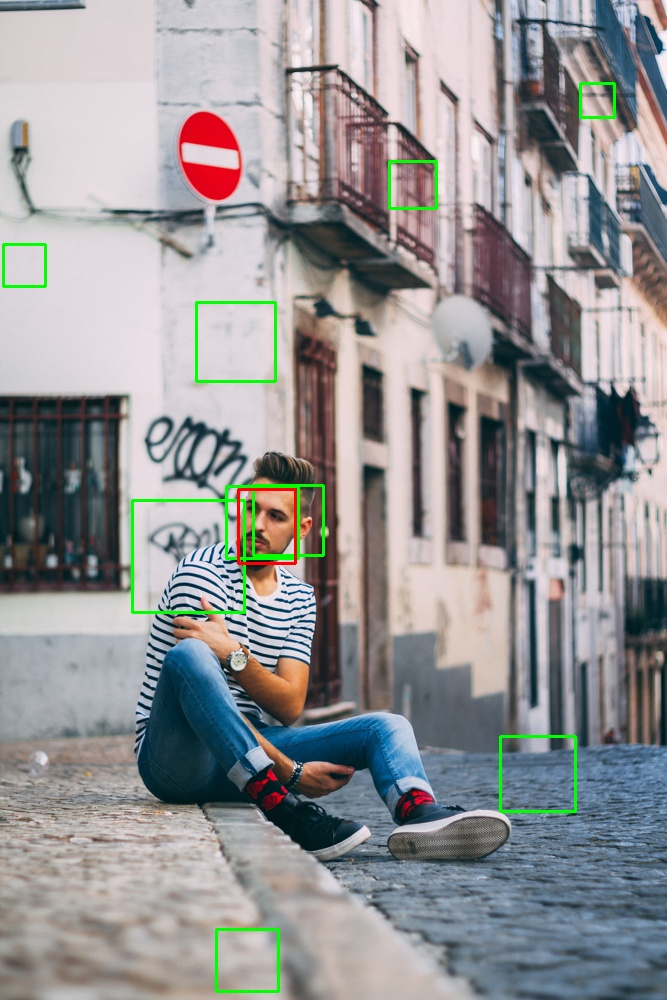
\includegraphics[height = 0.18\textheight]{images/NoEntry1.jpg}\label{fig:face1}}
  \hfill
  \subfloat[NoEntry5.jpg]{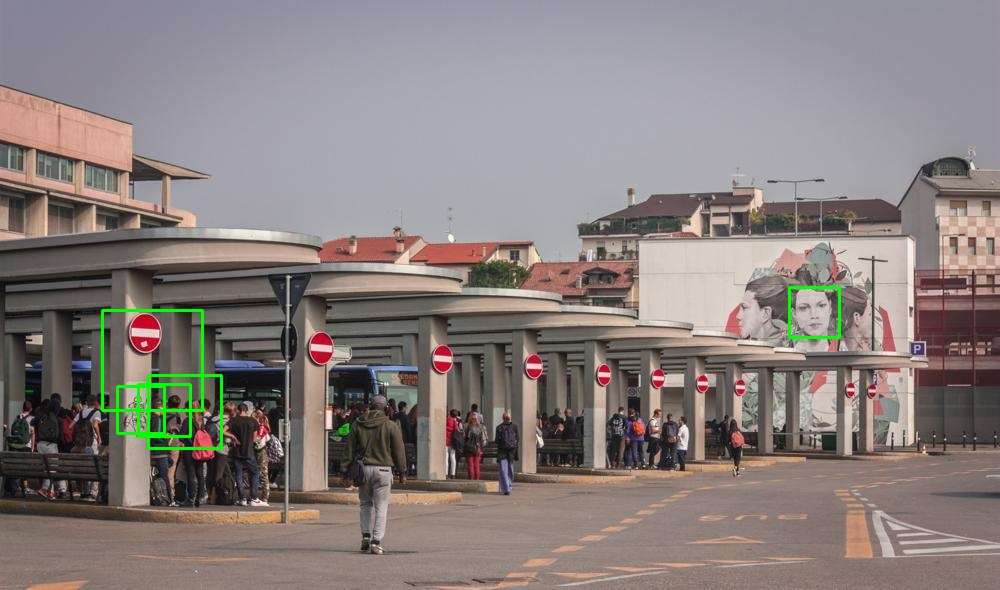
\includegraphics[height = 0.18\textheight]{images/NoEntry5.jpg}\label{fig:face5}}
  \hfill
  \subfloat[NoEntry11.jpg]{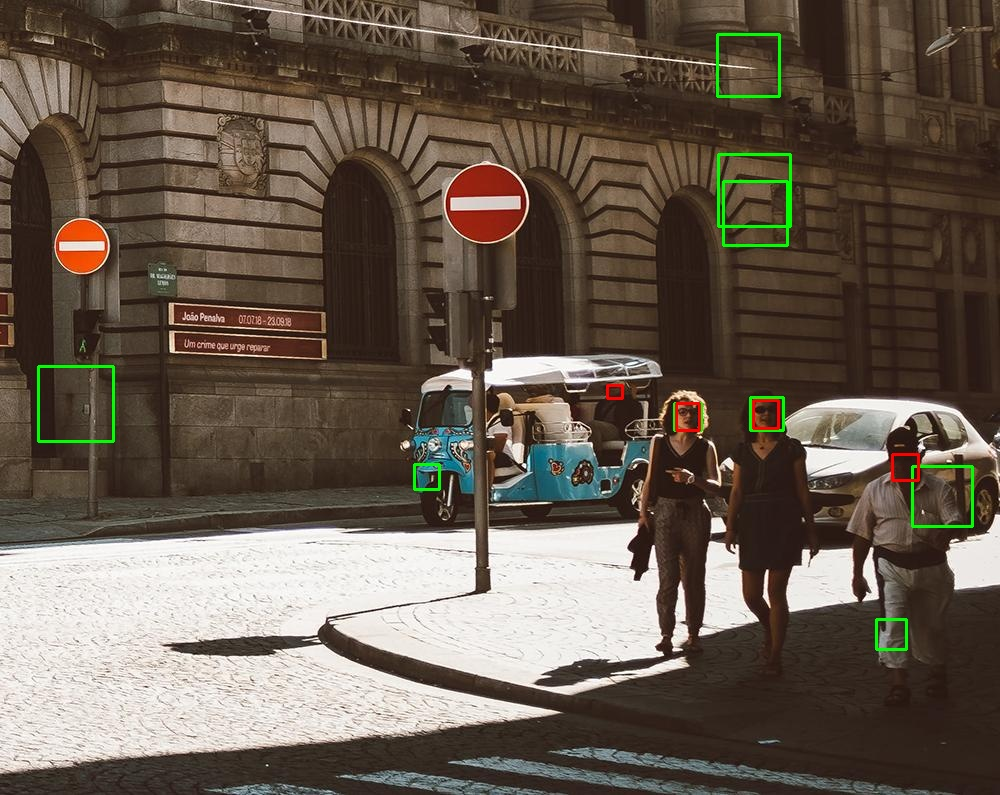
\includegraphics[height = 0.18\textheight]{images/NoEntry11.jpg}\label{fig:face11}}
  \hfill
  \subfloat[NoEntry2.jpg]{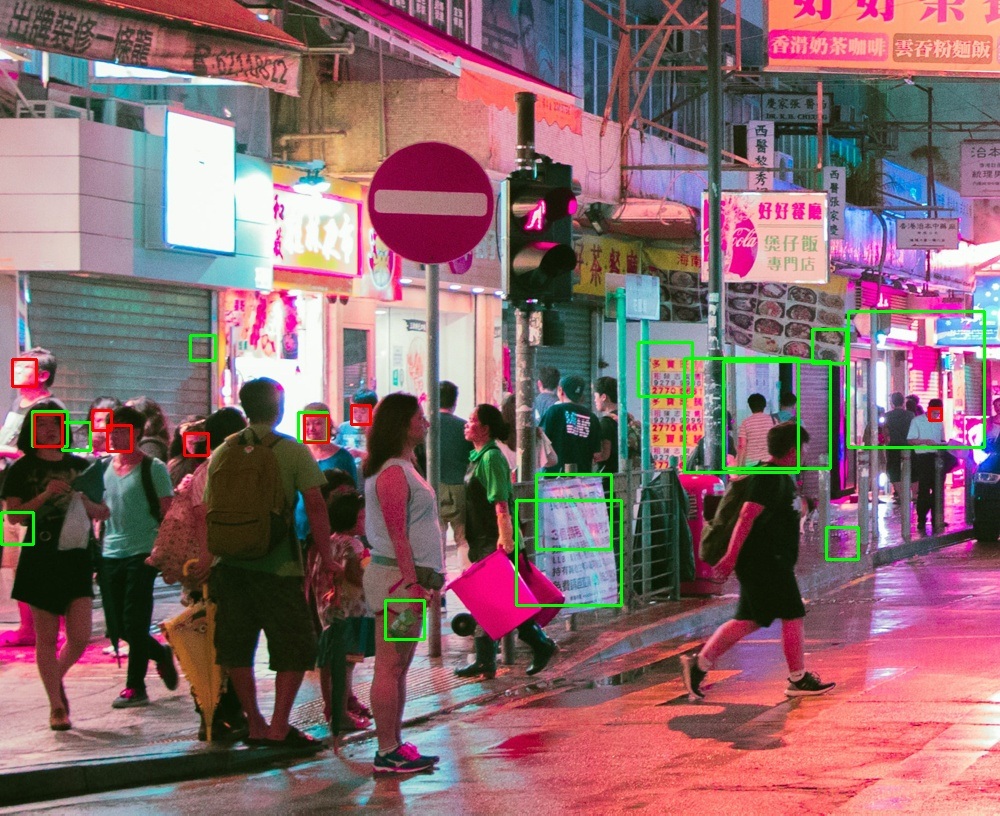
\includegraphics[height = 0.17\textheight]{images/NoEntry2.jpg}\label{fig:face2}}
  \hfill
  \subfloat[NoEntry4.jpg]{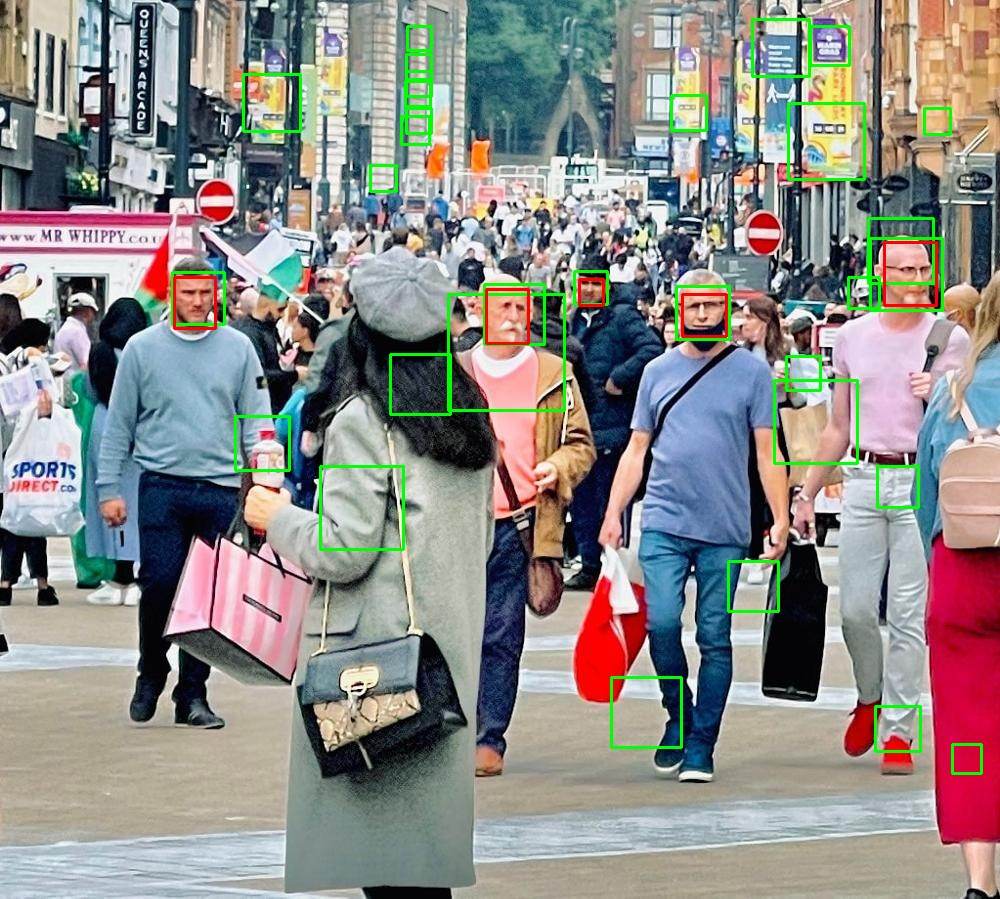
\includegraphics[height = 0.17\textheight]{images/NoEntry4.jpg}\label{fig:face4}}
  \hfill
  \subfloat[NoEntry7.jpg]{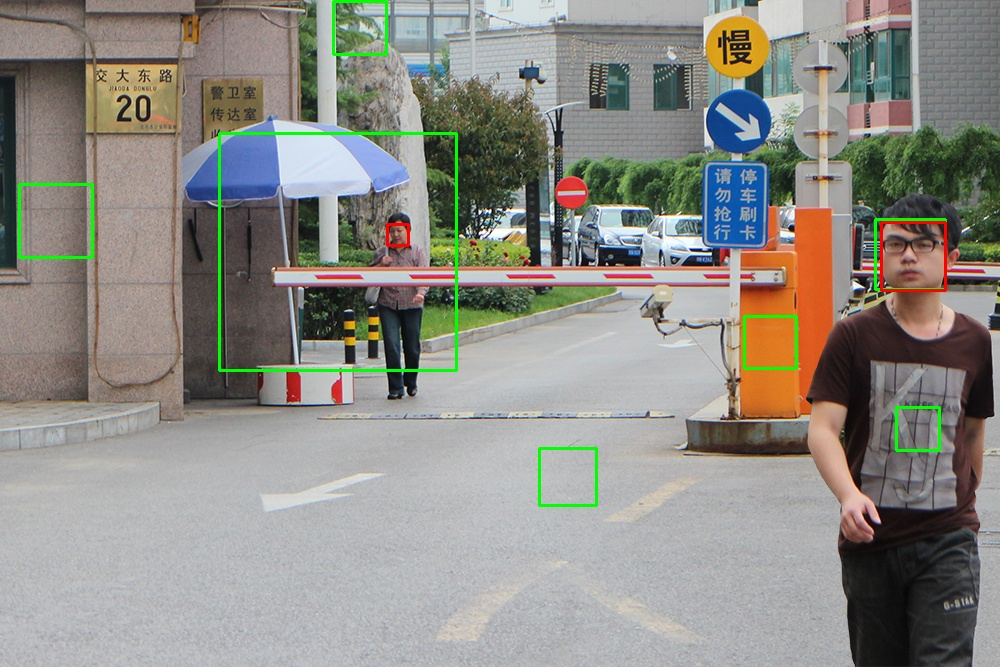
\includegraphics[height = 0.17\textheight]{images/NoEntry7.jpg}\label{fig:face7}}
  \caption{Six images with the bounding boxes of the ground truths (in red) and actually detected instances (in green) from the frontal face detector}\label{fig:face}
\end{figure}

\subsection{IOU, TPR and F\textsubscript{1} score}

\begin{wraptable}{r}{0.45\textwidth}
  \begin{center}
  \caption{True positive rate and F\textsubscript{1} score of the frontal face detector on each image}\label{tab:face}
  \begin{tabular}{l l l} 
    \hline\hline
    Filename & True positive rate & F\textsubscript{1} score\\
    \hline
    NoEntry0.jpg & Undefined & 0.00 \\ 
    NoEntry1.jpg & 1.00 & 0.20 \\ 
    NoEntry2.jpg & 0.25 & 0.18 \\ 
    NoEntry3.jpg & Undefined & Undefined \\ 
    NoEntry4.jpg & 1.00 & 0.28 \\ 
    NoEntry5.jpg & Undefined & 0.00 \\ 
    NoEntry6.jpg & Undefined & 0.00 \\ 
    NoEntry7.jpg & 0.50 & 0.22 \\ 
    NoEntry8.jpg & Undefined & 0.00 \\ 
    NoEntry9.jpg & Undefined & 0.00 \\ 
    NoEntry10.jpg & Undefined & 0.00 \\ 
    NoEntry11.jpg & 0.50 & 0.31 \\ 
    NoEntry12.jpg & Undefined & 0.00 \\ 
    NoEntry13.jpg & Undefined & 0.00 \\ 
    NoEntry14.jpg & Undefined & 0.00 \\ 
    NoEntry15.jpg & Undefined & 0.00 \\ 
    \hline
  \end{tabular}
  \end{center}
\end{wraptable} 

When assessing the true positive rate (TPR), the first practical difficulty that arises is how to define a bounding box as being positive.
I opted to define bounding boxes as positive if they had an intersection-over-union value of 50\% or greater.

On any detection task, it is possible to achieve a TPR of 100\% by detecting everything as positive.
By doing so, it eliminates the chance of there being any false negatives. 
Since TPR is defined as \[\text{TPR} = \frac{\text{TP}}{\text{TP} + \text{FN}}\]
if you eliminate all false negatives (i.e. $\text{FN} = 0$), the fraction will become
\[\text{TPR} = \frac{\text{TP}}{\text{TP} + 0} = \frac{\text{TP}}{\text{TP}} = 1\]
thus providing you with a TPR of 100\%.

\clearpage

\section{Building and testing my own detector}

\subsection{Training performance}

ROC graph
% \begin{tikzpicture}
% \begin{axis}[]
% \addplot+[
%   only marks,
%   % mark size=2.9pt
% ]
% table[]
% {fpr_tpr.dat};
% \end{axis}
% \end{tikzpicture}

\subsection{Testing performance}

\section{Integration with shape detectors}

\section{Improving my detector}



\clearpage
\begin{thebibliography}{9}
\end{thebibliography}
    

\end{document}